\documentclass[
  bibliography=totoc,     % Literatur im Inhaltsverzeichnis
  captions=tableheading,  % Tabellenüberschriften
  titlepage=firstiscover, % Titelseite ist Deckblatt
]{scrartcl}

% Paket float verbessern
\usepackage{scrhack}

% Warnung, falls nochmal kompiliert werden muss
\usepackage[aux]{rerunfilecheck}

% unverzichtbare Mathe-Befehle
\usepackage{amsmath}
% viele Mathe-Symbole
\usepackage{amssymb}
% Erweiterungen für amsmath
\usepackage{mathtools}

% Fonteinstellungen
\usepackage{fontspec}
% Latin Modern Fonts werden automatisch geladen
% Alternativ:
%\setromanfont{Libertinus Serif}
%\setsansfont{Libertinus Sans}
%\setmonofont{Libertinus Mono}
\recalctypearea % Wenn man andere Schriftarten gesetzt hat,
% sollte man das Seiten-Layout neu berechnen lassen

% deutsche Spracheinstellungen
\usepackage{polyglossia}
\setmainlanguage{german}


\usepackage[
  math-style=ISO,    % ┐
  bold-style=ISO,    % │
  sans-style=italic, % │ ISO-Standard folgen
  nabla=upright,     % │
  partial=upright,   % ┘
  warnings-off={           % ┐
    mathtools-colon,       % │ unnötige Warnungen ausschalten
    mathtools-overbracket, % │
  },                       % ┘
]{unicode-math}

% traditionelle Fonts für Mathematik
\setmathfont{Latin Modern Math}
% Alternativ:
%\setmathfont{Libertinus Math}

\setmathfont{XITS Math}[range={scr, bfscr}]
\setmathfont{XITS Math}[range={cal, bfcal}, StylisticSet=1]

% Zahlen und Einheiten
\usepackage[
  locale=DE,                   % deutsche Einstellungen
  separate-uncertainty=true,   % immer Fehler mit \pm
  per-mode=symbol-or-fraction, % / in inline math, fraction in display math
]{siunitx}

% chemische Formeln
\usepackage[
  version=4,
  math-greek=default, % ┐ mit unicode-math zusammenarbeiten
  text-greek=default, % ┘
]{mhchem}

% richtige Anführungszeichen
\usepackage[autostyle]{csquotes}

% schöne Brüche im Text
\usepackage{xfrac}

% Standardplatzierung für Floats einstellen
\usepackage{float}
\floatplacement{figure}{htbp}
\floatplacement{table}{htbp}

% Floats innerhalb einer Section halten
\usepackage[
  section, % Floats innerhalb der Section halten
  %below,   % unterhalb der Section aber auf der selben Seite ist ok
]{placeins}

% Seite drehen für breite Tabellen: landscape Umgebung
\usepackage{pdflscape}

% Captions schöner machen.
\usepackage[
  labelfont=bf,        % Tabelle x: Abbildung y: ist jetzt fett
  font=small,          % Schrift etwas kleiner als Dokument
  width=0.9\textwidth, % maximale Breite einer Caption schmaler
]{caption}
% subfigure, subtable, subref
\usepackage{subcaption}

% Grafiken können eingebunden werden
\usepackage{graphicx}
% größere Variation von Dateinamen möglich
\usepackage{grffile}

% schöne Tabellen
\usepackage{booktabs}

% Verbesserungen am Schriftbild
\usepackage{microtype}

% Literaturverzeichnis
\usepackage[
  backend=biber,
]{biblatex}
% Quellendatenbank
\addbibresource{lit.bib}
\addbibresource{programme.bib}

% Hyperlinks im Dokument
\usepackage[
  unicode,        % Unicode in PDF-Attributen erlauben
  pdfusetitle,    % Titel, Autoren und Datum als PDF-Attribute
  pdfcreator={},  % ┐ PDF-Attribute säubern
  pdfproducer={}, % ┘
  colorlinks
]{hyperref}
% erweiterte Bookmarks im PDF
\usepackage{bookmark}

%erweiterte Aufzählungen
\usepackage{paralist}

% Trennung von Wörtern mit Strichen
\usepackage[shortcuts]{extdash}

\author{%
  Lukas Rolf%
  \texorpdfstring{%
    \\%
    \href{mailto:lukas.rolf@tu-dortmund.de}{lukas.rolf@tu-dortmund.de}
  }{}%
  \texorpdfstring{\and}{, }%
  Yannik Brune%
  \texorpdfstring{%
    \\%
    \href{mailto:yannik.brune@tu-dortmund.de}{yannik.brune@tu-dortmund.de}
  }{}%
}
%\publishers{TU Dortmund – Fakultät Physik}


\subject{V301}
\title{EMK und Innenwiderstand von Spannungsquellen}
\date{
	Durchführung: DATUM
	\hspace{4em}
	Abgabe: DATUM
}

\begin{document}
	\maketitle
	\newpage
	\tableofcontents
	\newpage
	\newpage
	
	
	
	\begin{itemize}
		\item[a)] $1+1=2$
		\item[b)] $1-1=0$
		\item[c)] $\symbf{M}^\top \cdot \symbf{M}$
	\end{itemize}
	\begin{description}
		\item[Lukas] ist nicht anwesend!
	\end{description}
	\begin{enumerate}
		\item hallo
		\item ich 
		\item bin
		\item nicht
		\item da
		\item !
		\item mist
		\item steve
		\begin{figure}
			Hello i'm stupid 2 s.~\cite{wingate}
		\end{figure}
		Hello i'm stupid 3 7
	\end{enumerate}
	\begin{displaymath}
		\begin{pmatrix*}[r]
		1 & 1 & -4 \\
		-2 & 2 & 5\\
		1 & -3 & 6 \\
		-1 & 3 & -4 \\
		-1 & -45 & -3
		\end{pmatrix}
	\end{displaymath}
	\begin{table}
		a & b & c \\
		s & c & 3
	\end{table}
	\begin{table}
		\centering
		\caption{Eine schöne Tabelle mit Messdaten.}
		\label{tab:some_data}
		\sisetup{table-format=1.2}
		\begin{tabular}{S[table-format=3.0] S S S S[table-format=3.2]}
			\toprule{$f$} & {$l_\text{start}$} & {$l_1$} & 	{$l_{\text{kor},1}$} & {$B_1$} \\
			\midrule
			100 & 1.14 & 3.51 & 0.00 &   4.30 \\
			200 & 1.30 & 4.99 & 0.06 &  25.98 \\
			300 & 1.27 & 1.42 & 0.13 &  41.14 \\
			400 & 1.28 & 1.47 & 0.20 &  54.76 \\
			500 & 1.21 & 1.70 & 0.25 & 168.73 \\
			\bottomrule
		\end{tabular}
	\end{table}
	
	
\section{Theorie}
\label{sec:Theorie}

\subsection{Das Absorptionsgesetz}
Falls ein Teilchenstrahl durch Materie läuft, können die Teichen mit der Materie wechselwirken, sodass immer weniger Teilchen weiter ins Material vordringen. Dieser Abfall ist im Idealfall exponentiell. Das exponentielle Verhalten kommt dadurch zustande, dass angenommen wird, dass pro infinitesimalen Wegstückchen $\diff x$ in Richtung des Strahles immer der selbe Anteil der Teilchen absorbiert wird. Der Wirkungsquerschnitt $\sigma$ gibt an, wie groß die Wahrscheinlichkeit pro Materieteilchen pro Volumen $n$ und infinitesimalen Wegstückchen $\diff x$ ist, dass ein einfallendes Teilchen wechselwirkt bzw. absorbiert wird. Durch Multiplikation mit der Teilchenzahl im Strahl, die pro Zeiteinheit auf die Schicht treffen $N(x)$ und Integration über $\diff x$ ergibt sich die Anzahl der Wechselwirkungen pro Zeiteinheit $W(x)$. Unter der Annahme, dass ein Teilchen absorbiert wird falls es mit der Materie wechselwirkt ergibt sich durch Subtraktion von der ursprünglichen Teilchenanzahl $N_0$
\begin{equation}
	N(x)=N_0-W(x)=N_0 \exp(-n \sigma x)\text{.}
\end{equation}
Dieser Zusammenhang wird als Absorptionsgesetz bezeichnet. 
Der Faktor $n \sigma$ wird häufig mit dem sogenannten Absorptionskoeffizienten
\begin{equation}
	\mu = n \sigma
\end{equation}
abgekürzt. Mit einem bekannten $n$ lässt sich $\sigma$ leicht aus $\mu$ berechnen.
Es gilt die Beziehung
\begin{equation}
	\sigma = \frac{\mu}{n}=\frac{\mu}{\frac{z N_\text{A} \rho}{M}}=\frac{\mu M}{z N_\text{A} \rho}\text{,}\label{eq:HJHKJ}
\end{equation}
wobei $z$ die Ordnungszahl, $N_\text{A}$ die Avogadro-Konstante, $M$ das Molekulargewicht und $\rho$ die Dichte der Moleküle der Materie, in der die Absorption stattfindet (dem Absorbermaterial) ist.

\subsection{\texorpdfstring{Entstehung und Absorptionsverhalten von $\gamma$-Strahlung}{}}
In einem Atom können die einzelnen Elektronen sowie der Kern in einen angeregten Zustand versetzt werden. Die Elektronen z.B. durch Stoßvorgängen mit freien Elektronen und die Kerne z.B. bei Kernzerfällen. Diese Zustände sind quantisiert. Nach einiger Zeit gehen sie von einem angeregten Zustand $E_1$ zu einem mit geringerer Energie $E_2$ über. Dabei geben sie die Energie 
\begin{equation}
	E_\gamma=E_1-E_2
\end{equation}
in Form von einem $\gamma$-Quant ab. Die Frequenz $f$ und Wellenlänge $\lambda$ berechnen sich gemäß der Quantentheorie nach
\begin{equation}
	E_\gamma = h f = \frac{h c}{\lambda} \text{.}
\end{equation}
Hierin ist $h$ das Plancksche Wirkungsquantum und $c$ die Lichtgeschwindigkeit. 

Die $\gamma$-Quanten können mit den Elektronen, den Atomkernen und deren elektrischen Feldern wechselwirken. Es werden nur solche betrachtet, welche bei den üblichen Werten von $E_\gamma = \SI{10}{\kilo\electronvolt}$ bis $E_\gamma = \SI{10}{\mega\electronvolt}$ \cite{V704} am wahrscheinlichsten sind. Es kann sich dabei um drei verschiedenen Arten von Wechselwirkungen handeln: dem Annihilationsprozessen, der inelastischen Streuung und der elastischen Streuung. Bei Annihilationsprozessen verschwindet das $\gamma$-Quant, bei inelastischer Streuung gibt das $\gamma$-Quant einen Teil seiner Energie ab und seine Richtung ändert sich und bei elastischer Streuung ändert das $\gamma$-Quant seine Richtung ohne Energie abzugeben. Die wichtigsten auftretenden Effekte sind der Photo-Effekt, der Compton-Effekt und die Paarbildung.
Beim Photo-Effekt tritt Annihilation auf. Es wird die gesamte Energie des $\gamma$-Quants an ein gebundenes Elektron abgegeben, wobei das Elektron ungebunden wird und danach eine kinetische Energie von $E_\text{e} = h f - E_\text{B}$ besitzt. Hierbei ist $E_\text{B}$ die Bindungsenergie des Elektrons. Dieser Effekt tritt nur auf wenn $E_\gamma \ge E_\text{B}$ gilt. Die Wahrscheinlichkeit, dass ein $\gamma$-Quant absorbiert nimmt mit steigendem $z$ zu und fällt für steigende $E_\gamma \ge E_\text{B}$ ab. 
Beim Compton-Effekt wird ein $\gamma$-Quant an einem praktisch freien Elektron inelastisch gestreut. Dabei kann ein $\gamma$-Quant immer nur einen Teil seiner Energie abgeben. Eine schematische Darstellung ist in Abbildung \ref{fig:com} dargestellt.
\begin{figure}
	\centering
	\caption{Die schematische Darstellung des Compton-Effektes \cite{V704}.}
	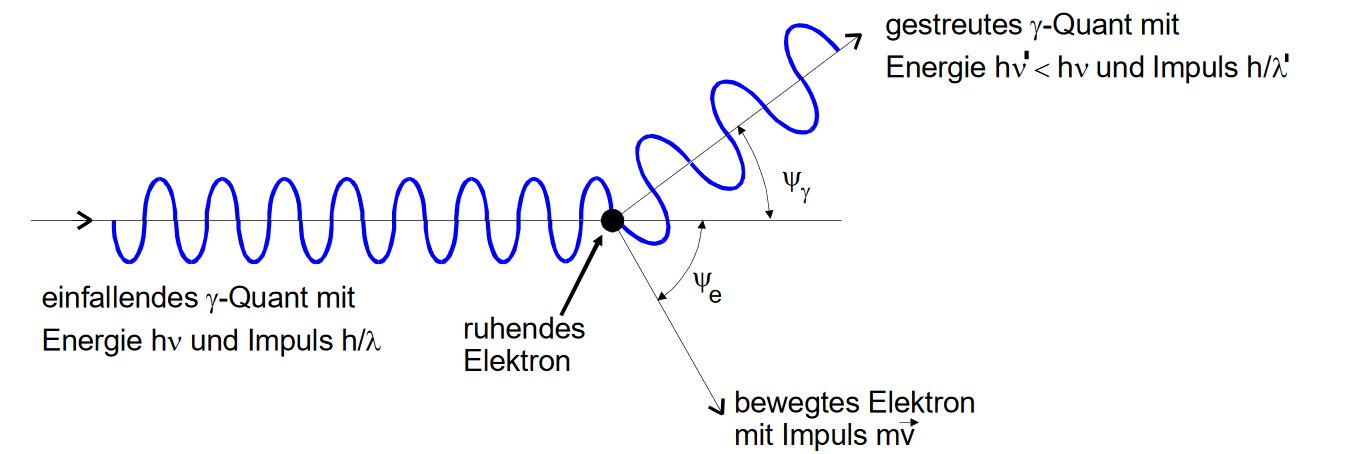
\includegraphics[width=\linewidth,height=\textheight-170pt,keepaspectratio]{content/images/com.png}
	\label{fig:com}
\end{figure}
Für den Wirkungsquerschnitt von der Compton-Streuung gilt
\begin{equation}
\sigma_\text{com} = 2 \pi r_\text{e}^2 \left\{ \frac{1+\epsilon}{\epsilon^2} \left[\frac{2 (1+\epsilon)}{1+2 \epsilon} -\frac{1}{\epsilon} \ln(1+ 2 \epsilon)\right] + \frac{1}{2 \epsilon} \ln(1 + 2 \epsilon) -\frac{1 + 3 \epsilon}{(1+2\epsilon)^2} \right\}\label{eq:HJHJ}
\end{equation}
mit dem klassischen Elektronenradius
\begin{equation}
	r_\text{e} = \frac{e_0^2}{4 \pi \epsilon_0 m_0 c^2} \approx \SI{2.82e-15}{\meter}
\end{equation}
und dem Verhältnis $\epsilon = E_\gamma / (m_0 c^2)$.
Hierin sind $m_0$ die Ruhemasse des Elektrons, $e_0$ die Elementarladung und $\epsilon_0$ die Influenzkonstante. Dieser Ausdruck für $\sigma_\text{com}$ vereinfacht sich für $E_\gamma \ll m_0 c^2$ zu
\begin{equation}
	\sigma_\text{com} \approx \frac{8}{3} \pi r_\text{e}^2 = \sigma_\text{Th} \text{.}
\end{equation}
Dabei wird $\sigma_\text{Th}$ als Thomsonscher Wirkungsquerschnitt bezeichnet.
Für $E_\gamma \gg m_0 c^2$ ist $\sigma_\text{com} \propto 1/\epsilon$. 
Bei der Paarbildung kann ein $\gamma$-Quant ein Elektron und ein Positron erzeugen. Dieser Effekt kann nur auftreten falls die Energie vom $\gamma$-Quant $E_\gamma > 2 m_o c^2$ ist und ein Teil des Impulses auf ein weiteres Teilchen übertragen werden kann. Dabei wird das $\gamma$-Quant annihiliert und die zusätzliche Energie in die kinetische Energie der Teilchen umgewandelt. Aus der Quantentheorie folgt, dass $\sigma_\text{p} \propto z^2$ ist.
Alle Effekte überlagern sich und bilden ein Verlauf von $\sigma$ der insbesondere von $E_\gamma$ abhängt. Für das Material Germanium ist dieser in Abbildung \ref{fig:kurve1} dargestellt.
\begin{figure}
	\centering
	\caption{Darstellung der Abhängigkeit des Absorptionskoeffizienten von der Energie und die Anteile der einzelnen Effekte an diesem für Germanium \cite{V704}.}
	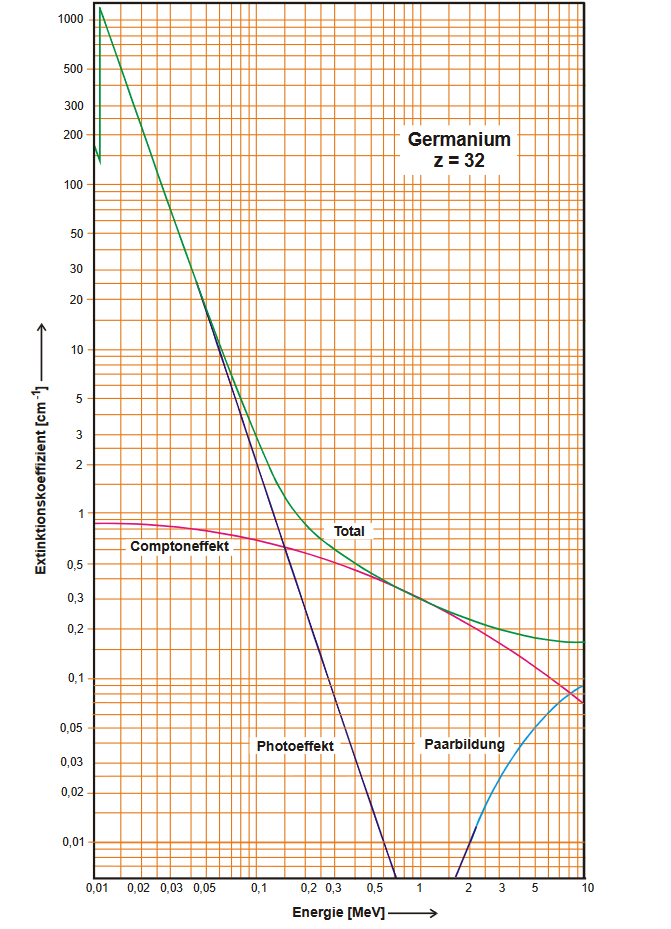
\includegraphics[width=\linewidth-170pt,height=\textheight-170pt,keepaspectratio]{content/images/kurvenverlauf1.png}
	\label{fig:kurve1}
\end{figure}

\subsection{\texorpdfstring{Entstehung und Absorptionsverhalten von $\beta$-Strahlung}{}}
$\beta$-Strahlung besteht aus $\beta$-Teilchen, welche durch Umwandlung eines Nukleons in einem Atomkern erzeugt und danach emittiert werden.
Die Umwandlung des Nukleons folgt entweder dem Reaktionsschema
\begin{equation}
 n \to p + \beta^- +\overline{\nu}_e
\end{equation}
oder 
\begin{equation}
p \to n + \beta^+ +\nu_e\text{.}
\end{equation}
Die dabei freiwerdende Energie $E_\text{f}$ verteilt sich statistisch auf die entstehenden Teilchen, sodass das Energiespektrum kontinuierlich ist. Die maximale Energie die ein $\beta$-Teilchen erhalten kann $E_\text{max}$ entspricht der freiwerdende Energie $E_\text{f}$. Die Verteilung der Energien der $\beta$-Teilchen ist in Abbildung \ref{fig:eSpektrum} dargestellt.
\begin{figure}
	\centering
	\caption{Darstellung des Energiespektrums der $\beta$-Teilchen \cite{V704}.}
	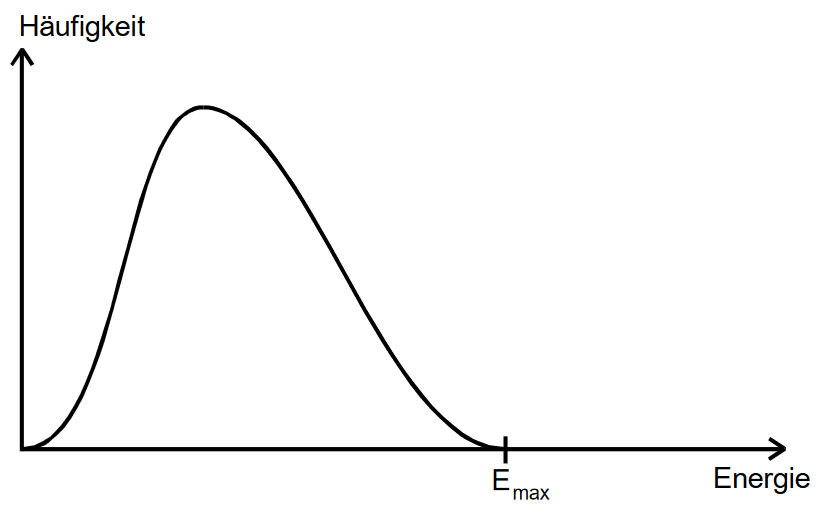
\includegraphics[width=\linewidth-170pt,height=\textheight-170pt,keepaspectratio]{content/images/emissionEnergie.png}
	\label{fig:eSpektrum}
\end{figure}
Die $\beta$-Teilchen werden im Material sowohl elastisch an den Atomkernen als auch inelastisch an den Atomkernen und Elektronen gestreut.
Die elastische Streuung an den Atomkernen führt zu staken Richtungsänderungen und längeren effektiven Wegen der $\beta$-Teilchen im Material, wie in Abbildung \ref{fig:verlaufTeilchen} dargestellt ist.
\begin{figure}
	\centering
	\caption{Beispielhafte Wege von einzelnen $\beta$-Teilchen in Materie \cite{V704}.}
	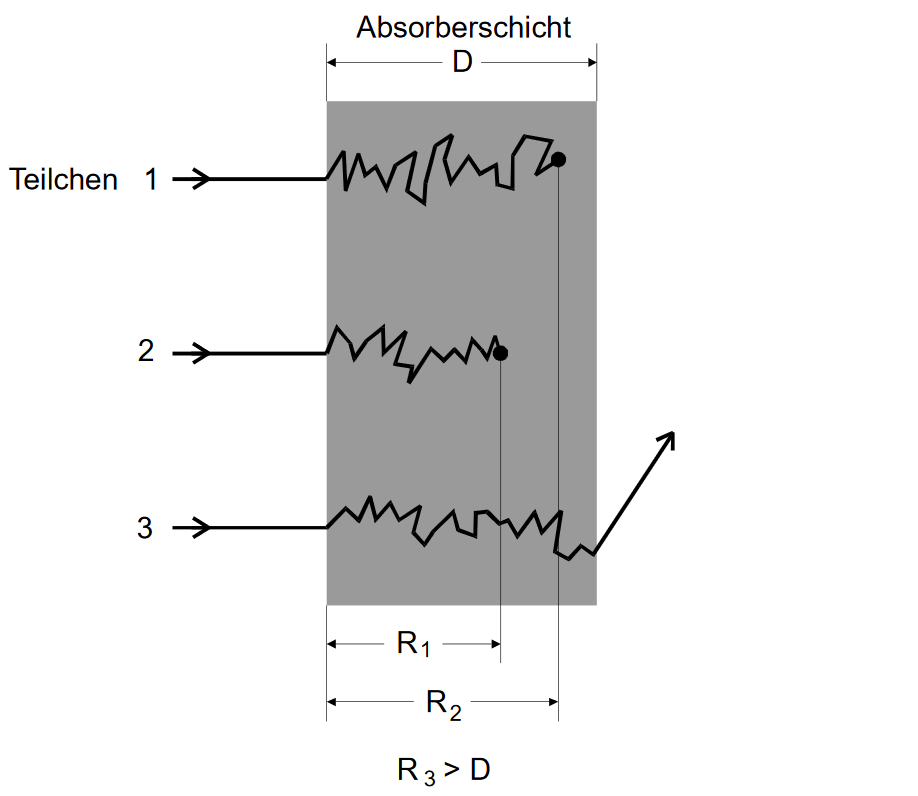
\includegraphics[width=\linewidth-170pt,height=\textheight-170pt,keepaspectratio]{content/images/verlaufTeilchen.png}
	\label{fig:verlaufTeilchen}
\end{figure}
Die inelastische Streuung an den Atomkernen tritt auf wenn sich die geladenen $\beta$-Teilchen durch die elektrischen Felder der Kerne bewegen und dadurch beschleunigt werden. Bei der Beschleunigung von geladenen Teilchen werden jedoch elektromagnetische Wellen abgestrahlt, was zu einem Energieverlust der Teilchen führt. Die enstehende Strahlung wird als Bremsstrahlung bezeichnet. Die Wahrscheinlichkeit, dass Bremsstrahlung auftritt ist durch den Wirkungsquerschnitt
\begin{equation}
\sigma_\text{Br}=\alpha r_\text{e}^2 z^2
\end{equation}
gegeben, wobei $\alpha\approx 1/137$ die Sommerfeldsche Feinstruckturkonstante ist. Für den mittleren Energieverlust einer $\beta$-Teilchen mit der Energie $E_\beta$ gilt
\begin{equation}
\overline{E_\text{Br}} \approx 7 10^{-7} z E_\beta^2 \text{.}
\end{equation}
Diese Näherung ist gültig für Energien bis etwa $\SI{2500}{\kilo\electronvolt}$.
Die Wahrscheinlichkeit einer inelastische Streuung der $\beta$-Teilchen durch Ionisation oder Anregung der Atome im Absorber wächst mit der Anzahl der Elektronen pro Volumen an. Dabei geben die $\beta$-Teilchen jeweils nur einen kleinen Teil ihrer Energie ab. Der Energieverlust der $\beta$-Teilchen pro Absorberschichtdicke ist für $\beta$-Teilchen mit $E_\beta < m_0 c^2$ durch
\begin{equation}
\frac{\diff E}{\diff x} \approx - \frac{2 \pi r_\text{e}^2}{E_\beta} \frac{N_\text{L} \rho}{M} z \ln\left(\frac{E_\beta}{I}\right)
\end{equation}
gegeben, wobei $I$ die Ionisierungsenergie ist.

Für die Absorbtionskurve von $\beta$-Strahlung eines natürlichen Strahlers ergibt sich eine Kurve der in Abbildung \ref{fig:kurvenverlauf2} dargestellten Form, wobei statt der Schichtdicke $D$ des Absorbers die Massenbelegung $R = \rho D$ aufgetragen ist. Aus dieser Absorptionskurve kann durch Näherung der linearen Anteile und Bestimmung des Schnittpunktes die maximale Reichweite $R_\text{max}$ der $\beta$-Teilchen bestimmt werden. Diese hängt mit der maximalen Energie der $\beta$-Teilchen $E_\text{max}$ zusammen. Im für den Versuch bedeutsamen Energiebereich gilt der Zusammenhang
\begin{equation}
	E_\text{max}=1.92 \sqrt{R_\text{max}^2 + 0.22 R_\text{max}}\text{ ,}\label{eq:HJKH}
\end{equation}
wobei $E_\text{max}$ in $\si{\mega\electronvolt}$ und $R_\text{max}$ in $\si{\gram\per\centi\meter\squared}$ ist.
Der Zusammenhang wurde empirisch bestimmt.









\begin{figure}
	\centering
	\caption{Absorptionskurve von $\beta$-Teilchen in Materie \cite{V704}.}
	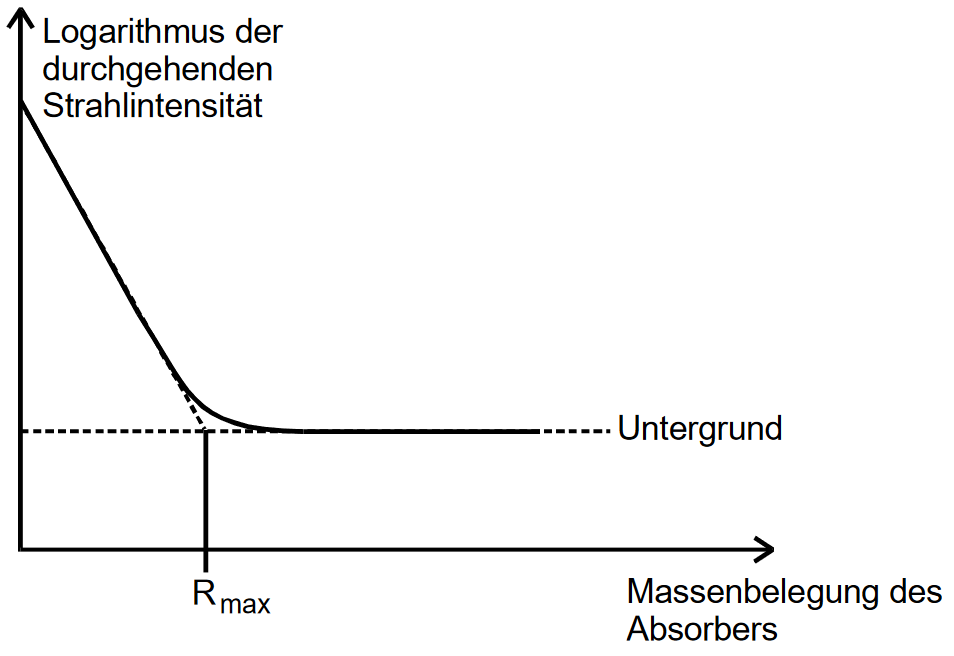
\includegraphics[width=\linewidth-170pt,height=\textheight-170pt,keepaspectratio]{content/images/kurvenverlauf2.png}
	\label{fig:kurvenverlauf2}
\end{figure}





	
\section{Durchführung}
\label{sec:Durchführung}
Als erstes werden die Längen aller Acrylzylinder mit einer Schieblehre vermessen.
Der allgemeine Gain wird so eingestellt, dass die resultierenden Peaks eines AScans im Impuls Echo-Verfahren
noch komplett sichtbar sind.
Im Anschluss wird zunächst das Impuls-Echo-Verfahren an den Zylindern erprobt.
Hierzu wird der Zylinder auf ein Papiertaschentuch gestellt. Anschließend wird eine Sonde
 mithilfe von bidestiliertem Wasser von oben angekoppelt. Das Ultraschallechoskop
 wird so eingestellt, dass die verwendete Sonde sowohl als Sender als auch als Empfänger fungiert.
 Nun wird ein AScan durchgeführt und die Koordinaten der auftretenden Peaks, sowie der zugehörige Tgc-Wert, werden notiert.
 Dies wird für die anderen fünf Zylinderlängen wiederholt. Falls die auftretenden
 Peaks zu gering oder zu hoch ausfallen muss die TGC-Einstellung gegebenenfalls nachjustiert werden.
 Aus diesen lässt sich sowohl die Dämpfungskosntante als auch die
 Schallgeschwindigkeit in Acryl bestimmen.
 Als nächstes wird der Versuch nochmals mit dem Durchschallungsverfahren wiederholt.
 Hierzu wird der jeweilige Zylinder in eine Halterung gelegt und von beiden
 Seiten mit Koppelgel an jeweils eine Sonde angekoppelt. Die Eingänge des Ultraschallechoskops
 werden entsprechend eingestellt. Auch hier wird ein AScan durchgeführt und die
 entsprechenden Daten werden notiert.
 Nun wird eine spektrale Analyse sowie eine Cepstrumbestimmung durchgeführt. Hierzu
 werden zwei Acrylscheiben unterschiedlicher Dicke mit bidestiliertem Wasser gekoppelt.
 Die dünnere Scheibe liegt ganz unten. Um die auftretenden Peaks besser vom
 Anfangspeak an der Grenzschicht von Sonde und Acryl zu trennen wird ein Zylinder
 zwischen Sonde und Platten gekoppelt. Der Tgc wird so eingestellt, dass 3 Peaks zu erkennen sind.
 Die Curser werden so gesetzt, dass alle Peaks im Bereich zwischen ihnen liegen. Daraufhin wird eine
 FFT-Analyse über den entsprechenden Menüpunkt gestartet. Diese liefert Spektrum und Cepstrum.
 Auch hier werden die Koordinaten der Peaks notiert.
 Zuletzt wird ein Augenmodell untersucht. Hierzu wird wieder eine
 Sonde im Impuls-Echo-Verfahren mit Koppelgel an die künstliche Hornhaut des Modells angekoppelt
 und leicht bewegt bis ein Echo der Augenrückwand zu sehen ist. es werden wieder
 die Positionsdaten der Peaks notiert. Es ist darauf zu achten, dass kein übermäßiger
 Druck auf die Hornhaut ausgeübt wird, da das Augenmodell sonst beschädigt werden könnte.

	\section{Auswertung}
\label{sec:Auswertung}


Die Graphen wurden sowohl mit Matplotlib \cite{matplotlib} als auch NumPy \cite{numpy} erstellt. Die
Fehlerrechnung wurde mithilfe von Uncertainties \cite{uncertainties} durchgeführt.
Die Daten der Betrastrahlung stammen von einer Parallelgruppe.
\subsection{Die gemessenen Daten}

Es ist zu beachten, dass die gemessenen Aufschläge ein statistisches Verhalten
aufweisen und daher mit einem Fehler von
\begin{equation}
\sigma = \sqrt{N}
\end{equation}
behaftet sind. Daraus wird die Intensität mit
\begin{equation}
  I = \frac{N}{t} \pm \frac{\sigma}{t}
\end{equation}
 berechnet. Zusätzlich müssen die Treffer des Nulleffektes abgezogen werden,
welcher aufgrund von kosmischer Strahlung auftreten. Da die daraus folgenden
durchgehenden Intensitäten jedoch ungleich kleiner sind, werden die zugehörigen
 Fehler nicht berücksichtigt. Für die $\gamma$-Strahlung ergibt sich ein
 Nulleffekt von $\SI{1.001}{\per\second}$, für die $\beta$-Strahlung $\SI{0.514}{\per\second}$.

 \begin{table}
  \centering
  \caption{Die Materialeigenschaften der verwendeten Absorber.}
  \input{build/rohdaten.tex}
  \label{tab:rohd}
 \end{table}

\begin{table}
 \centering
 \caption{Die Absorptionsdaten der $\gamma$-Strahlung mit Kupfer als Absorber.}
 \input{build/tabgammakupfer.tex}
 \label{tab:k}
\end{table}

\begin{table}
 \centering
 \caption{Die Absorptionsdaten der $\gamma$-Strahlung mit Kupfer als Absorber.}
 \input{build/tabgammaeisen.tex}
 \label{tab:e}
\end{table}

\begin{table}
 \centering
 \caption{Die Absorptionsdaten der $\beta$-Strahlung mit Kupfer als Absorber.}
 \input{build/tabgammabetaJ.tex}
 \label{tab:betaJ}
\end{table}

\subsection{\texorpdfstring{Bestimmung der Absorptionskoeffizienten und der Ausgangsstrahlung mithilfe von $\gamma$-Absorptionskurven}{}}

\begin{figure}
 \centering
 \caption{Die halblogarithmische Darstellung der durchgehenden $\gamma$-Strahlintensität gegenüber der Schichtdicke des Kupferabsorbers.}
 \includegraphics[width=\linewidth-70pt,height=\textheight-70pt,keepaspectratio]{build/Kupfer.pdf}
 \label{fig:kupfer}
\end{figure}

\begin{figure}
 \centering
 \caption{Die halblogarithmische Darstellung der durchgehenden $\gamma$-Strahlintensität gegenüber der Schichtdicke des Eisenabsorbers.}
 \includegraphics[width=\linewidth-70pt,height=\textheight-70pt,keepaspectratio]{build/Eisen.pdf}
 \label{fig:eisen}
\end{figure}

\begin{table}
 \centering
 \caption{Die Absorptionsdaten der $\beta$-Strahlung mit Aluminium als Absorber.}
 \input{build/tabgammabetaJ.tex}
 \label{tab:betaJ}
\end{table}

Zuerst wird das Absorptionsverhalten von Kupfer und Eisen unter der Gammastrahlung einer $^{137}$Cs-Quelle untersucht. Hierzu werden die Koeffizienten $\mu$ und $N(0)$ des Absorptionsgesetzes für beide Metalle bestimmt. Mithilfe einer halblogarithmischen Darstellung der zeitlich normierten Treffer gegenüber der Metalldicke ergeben sich die Graphen in  den Abb. \ref{fig:kupfer} und \ref{fig:eisen}. Damit folgen $\mu$ und $N(0)$ über eine Ausgleichsrechnung der Form
\begin{equation}
y = a x+ b \text{ mit } \mu = a \text{ und } N(0) = \exp(b)
\end{equation} Damit ergeben sich die experimentellen Ergebnisse in Tabelle \ref{tab:ergebnisse}.

\begin{table}
 \centering
 \caption{Die Ergebnisse der $\gamma$-Strahlungsabsorption.}
 \input{build/ergebnisse.tex}
 \label{tab:erg1}
\end{table}

\subsection{Vergleich mit den theoretischen Absorptionskoeffizienten}
Mithilfe der Formeln \ref{eq:HJHJ} und \ref{eq:HJHKJ} ergeben sich die theoretischen
Absorptionskoeffizienten. Auf Basis der Daten aus Tabelle \ref{tab:rohd} und einem
 $\epsilon$ von 1.295 \cite{V704} folgen die berechneten Koeffizienten in Tabelle \ref{tab:erg1}.
 Die Daten stammen für Kupfer von \cite{Kupfer}, für Eisen von \cite{Eisen}.
Es ist zu erkennen das die berechnete Absorption der beiden Metalle in beiden
Fällen größer ausfällt, als die experimentell gemessene. Daher ist davon auszugehen,
dass der Compton-Effekt bei beiden Absorptionen die einzige messbar auftretende Wechselwirkung.
Zusätzlich ist bei der Eisenmessung von einem systematischen Fehler auszugehen,
da dieser weitaus stärker nach unten abweicht. Die Ursachen sind in der Diskussion zu erörtern.
\subsection{Bestimmung der Maximalenergie von $^{99}$Tc }


\begin{figure}
 \centering
 \caption{Die halblogarithmische Darstellung der Treffer pro Sekunde gegenüber der Schichtdicke des Aluminiumabsorbers bei $\beta$-Strahlung}
 \includegraphics[width=\linewidth-70pt,height=\textheight-70pt,keepaspectratio]{build/BetaJ.pdf}
 \label{fig:betaj}
\end{figure}

Zuletzt wird die Maximalenergie der $\gamma$-Quanten von $^{99}$Tc über deren Absorption von Aluminium bestimmt. Hierzu werden
die durchgehende Strahlungsintensität halblogarithmisch gegen die Massenbelegung aufgetragen.
Mit den Daten aus Tabelle \ref{tab:betaJ} und einer Dichte von $\SI{2.699}{\gram\per\cubic\centi\meter}$ folgt der Graph in Abb. \ref{fig:betaj}. Anschließend werden
die beiden großteils linearen Bereiche der Kurve durch linearen Funktionen approximiert. Der
 Schnittpunkt beider Geraden bildet das gesuchte $R_\text{max}$. Mithilfe von Formel \ref{eq:HJKH}
 ergibt sich schließlich die Maximalenergie $E_\text{max}$. Mit den bestimmten Daten folgen daher die Parameter in Tabelle \ref{tab:erg2}.
\begin{table}
 \centering
 \caption{Die Ergebnisse der $\beta$-Strahlungsabsorption.}
 \input{build/ergebnisse2.tex}
 \label{tab:erg2}
\end{table}

	
\section{Diskussion}
\label{sec:Diskussion}

 \begin{table}
 	\centering
 	\caption{Ergebnisse.}
 	\input{build/tabs.tex}
 \end{table}

Die erstellten Kennlinien folgen dem in der Theorie \ref{fig:Kennlinie} dargestellten Verlauf.
 Auch die Kennlinie unter einem Heizstrom von $I_\text{f} = \SI{2.5}{\ampere}$
 besitzt einen Sättigungsstrom. Dieser konnte jedoch nicht ermittelt werden.
Die logarithmische Darstellung dieser Kennlinie zeigt leichte Schwankungen im
unteren und oberen Bereich der X-Achse. Dies folgt, da die Ausgleichsgerade auf
den Daten in der Mitte basiert, da dort das Raumladungsgebiet vermutet wird.
Die Strommessung im Anlaufstromgebiet zeigt, in der halblogarithmischen
Darstellung \ref{fig:Graphlog3}, Schwankungen. Möglichen Fehlerquellen sind im
Versuchsaufbau zu finden. Da sich die gemessenen Ströme im $\si{\nano\ampere}$
Bereich befinden, wird ein sehr empfindliches Messgerät mit Verstärker benötigt.
Dieses ist störanfällig und benötigt eine sehr kurze Leitung zwischen Anode und Eingang.
Zudem kommt es beim Amperemeter zu Schwankungen, wenn sich Objekte in der Nähe der
Leitung befinden. Zudem verfälscht der Übergangswiderstand zwischen Stecker und
Buchse das Ergebnis aufgrund seiner exponentiellen Spannungsabhängigkeit das Ergebnis.
 Er kann auch nicht komplett behoben werden. Eine zusätzliche Fehlerquelle sind
 Folgen der direkten Heizung. Abweichungen aufgrund des internen Widerstandes
 sind irrelevant klein. Aufgrund dessen liegt der hiermit bestimmte Temperaturwert
 deutlich über den per Heizleistung bestimmten Temperaturen. Die ermittelte
 Austrittsarbeit liegt $\SI{3}{\percent}$ über dem Literaturwert von $\SI{4.5}{\electronvolt}$ \cite{wolfaus}. Dies einspricht drei Standartabweichungen und kann durch einen der zuvor genannten Gründe zustande kommen. Auch nicht berücksichtigte Effekte und die Missachtung der Ablesefehler können dazu beitragen.

	\newpage
	
	\printbibliography
\end{document}
